\newpage
\subsection{Continuous Integration, Deployment und Delivery}\label{continouous_whatever}

Die Begriffe Continuous Integration, Deployment und Delivery sind eng miteinander verbunden und werden häufig als Abkürzung CI/CD verwendet.
Eine sogenannte CI/CD Pripeline besteht dabei aus mehreren ineinandergreifenden Komponenten: \footnote{Shweta et. al, vgl.~\cite{Shweta2014}~[S.214]} \\

\begin{figure}[htb]
    \centering
    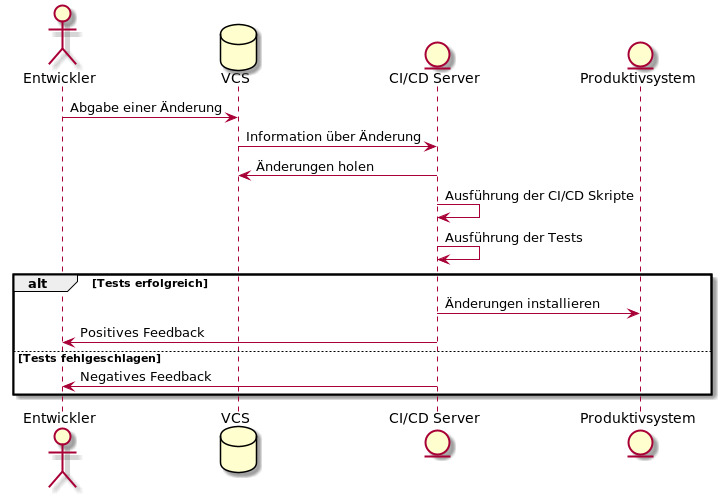
\includegraphics[width=1.0\textwidth]{images/cicd_pipeline.jpg}
    \caption[Vereinfachte CI/CD Pipeline]{Vereinfachte CI/CD Pipeline}
    \label{fig:Vereinfachte CI/CD Pipeline}
\end{figure}


%\begin{itemize}
%    \item \textbf{Entwickler:} Mitarbeiter die Quellcode verändern
%    \item \textbf{VCS:} Versionsverwaltung zur Zusammenarbeit am Code
%    \item \textbf{CI/CD Server:}
%    \item \textbf{CI/CD Skripte/Konfiguration:}
%    \item \textbf{Feedback:}
%    \item \textbf{Produktivsystem:}
%\end{itemize}


%- Versionskontrolle (VCS): Der Quellcode sollte in einem System zentral verwaltet werden.
%- CI Server: Ein System das die Änderungen aller Entwickler automatisch, zusammenführt, testet und je nach Konfiugration sogar ausrollt.
%- CI Skripte/Konfiguration: Einem CI Server muss per Skript oder Konfiguration mitgeteilt werden wie ein Projekt zu kompilieren, testen und zu deployen ist. In der Regel werden diese Skirpte zusammen mit dem Quellcode im VCS gehalten.
%- Feedback Mechanismen: Wenn ein Entwickler einen CI/CD Job started kann es unter Umständen einen Moment dauern bis das Ergebnis feststeht, daher sollte ein CI Server Benachrichtigungen in Form von E-Mails oder Kommentaren in dem entsprechenden VCS haben.
